\begin{figure}[ht]
    \begin{subfigure}[t]{.45\textwidth}
        \caption{}
        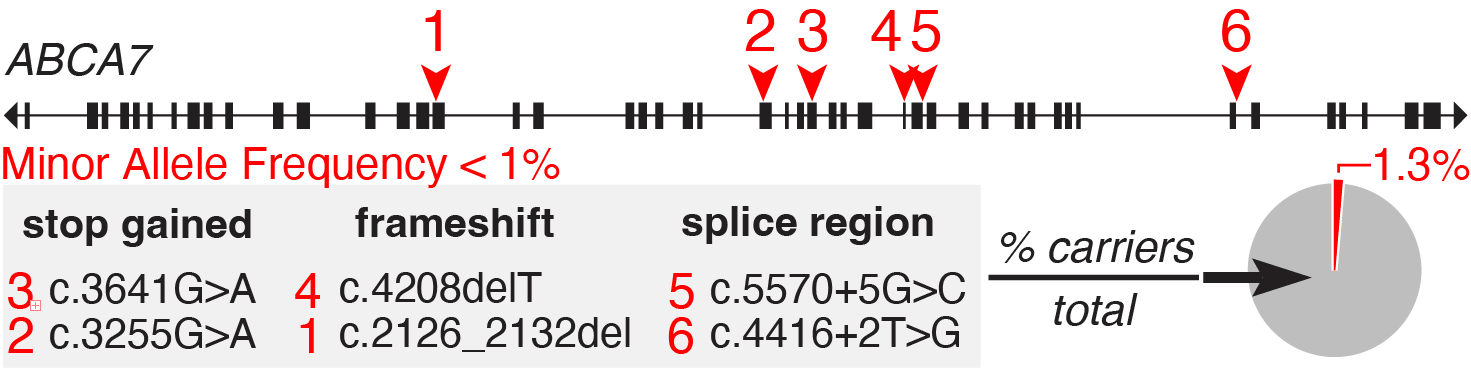
\includegraphics[width=\textwidth]{./main_plots/abca7_variants_cartoon.png}        
    \end{subfigure}
    \begin{subfigure}[t]{.55\textwidth}
        \caption{}
        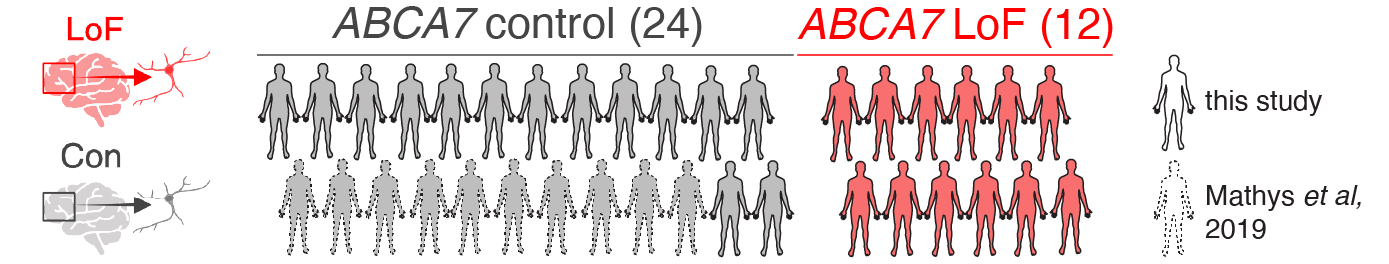
\includegraphics[width=\textwidth]{./main_plots/cohort_cartoon.png}        
    \end{subfigure}
    \\[-1ex] 
    \begin{subfigure}[t]{.5\textwidth}
        \begin{subfigure}[t]{\textwidth}
            \caption{}
            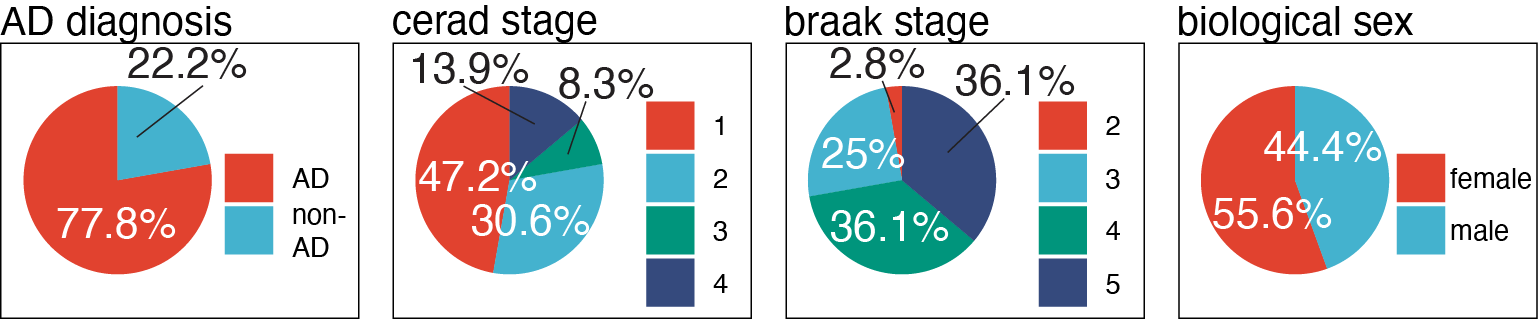
\includegraphics[width=\textwidth]{./main_plots/pie_charts.png}        
        \end{subfigure}
        \begin{subfigure}[t]{.45\textwidth}
            \caption{}
            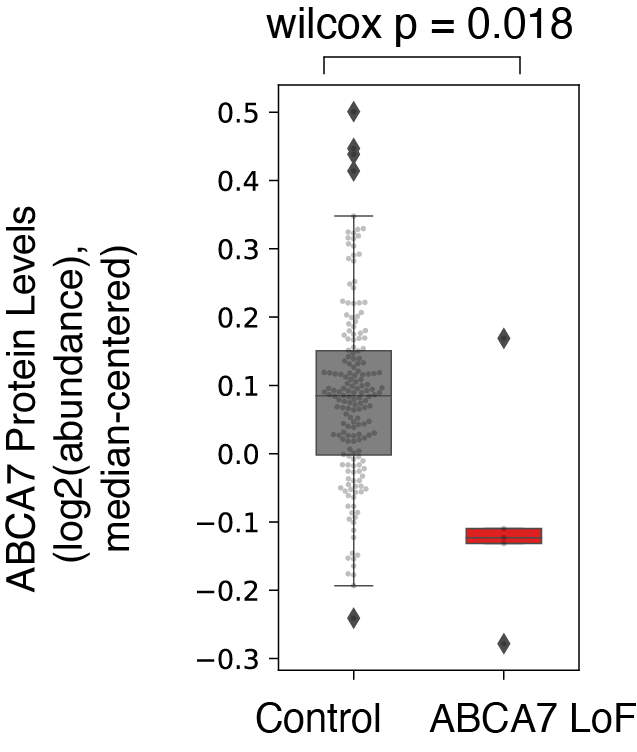
\includegraphics[width=\textwidth]{./main_plots/abca7_protein_levels.png}        
        \end{subfigure}
        \begin{subfigure}[t]{.5\textwidth}
            \caption{}
            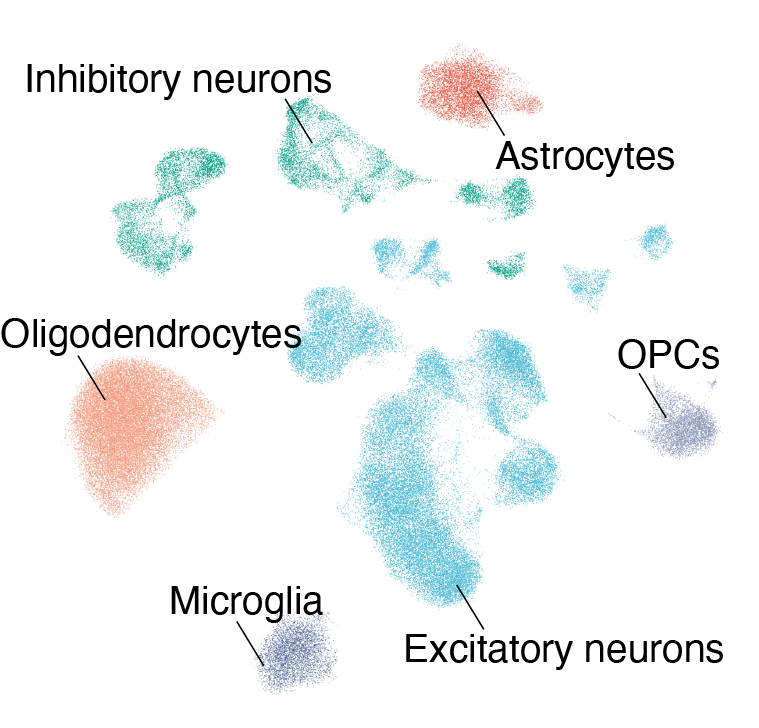
\includegraphics[width=\textwidth]{./main_plots/cell_projection.png}        
        \end{subfigure}
    \\[-3ex] 
    \end{subfigure}
    \begin{subfigure}[t]{0.5\textwidth}
        \caption{}
        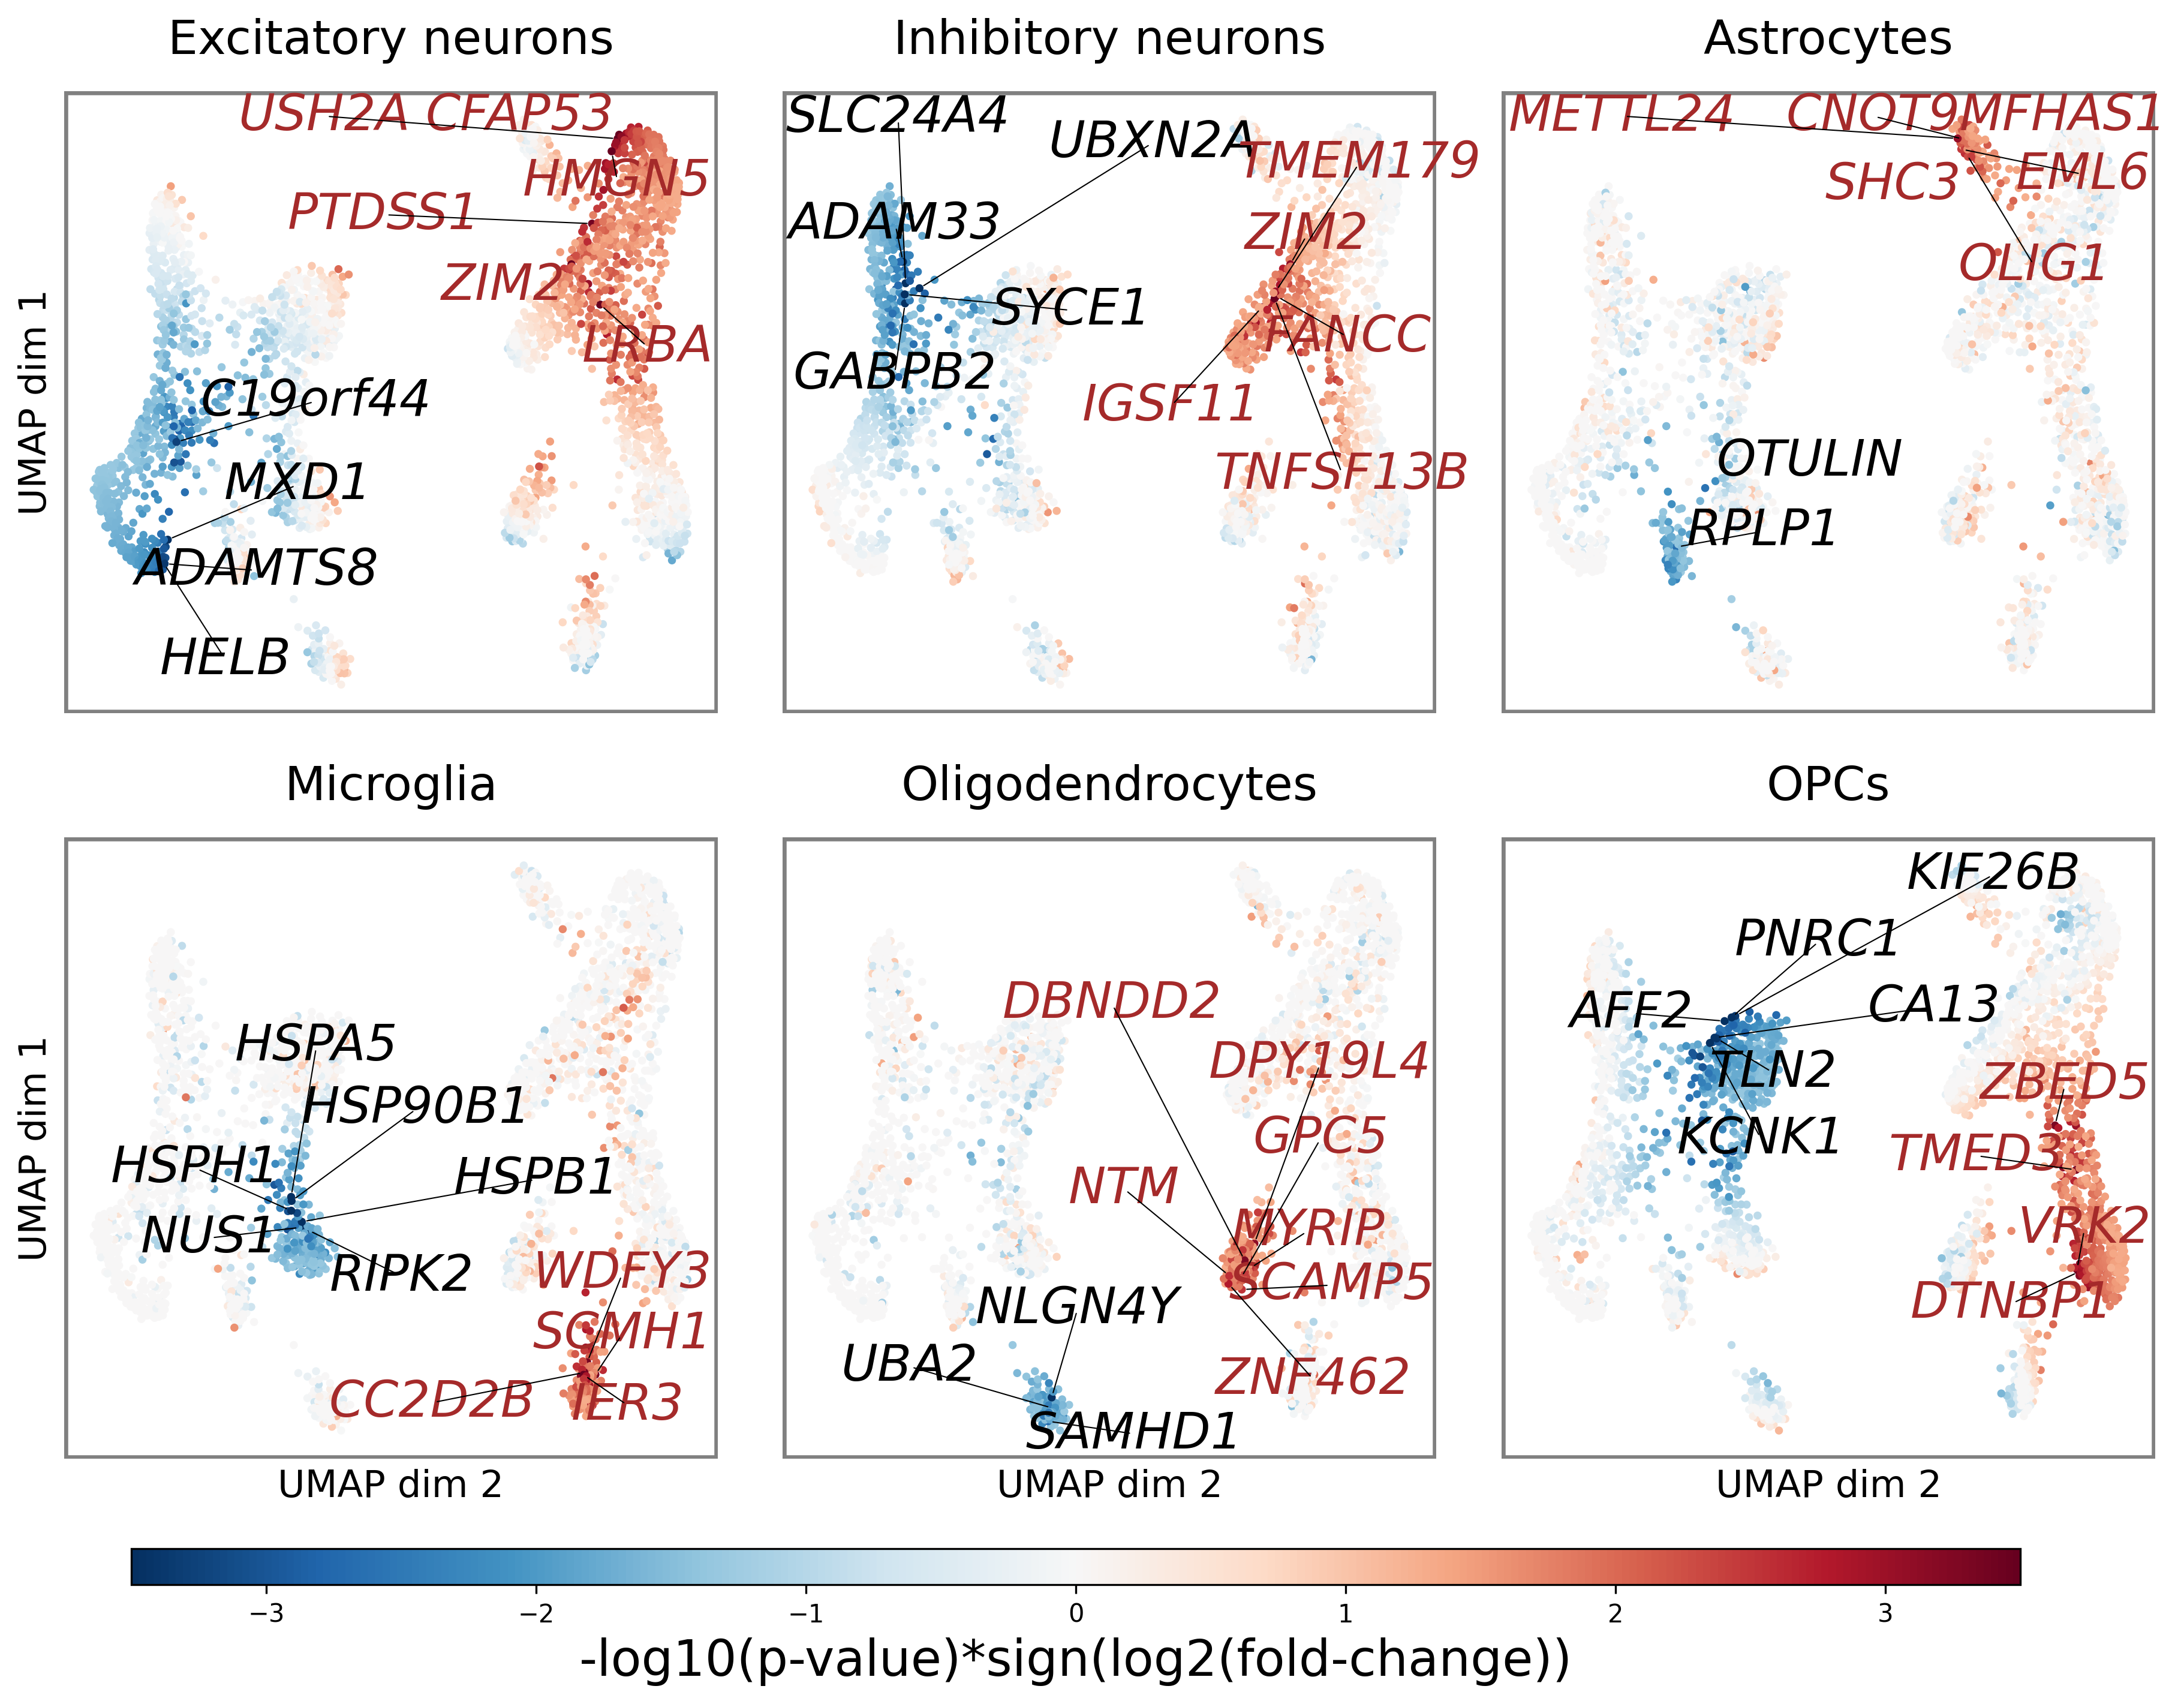
\includegraphics[width=\textwidth]{./main_plots/umap_projection_top_genes.png}        
    \end{subfigure}
    \begin{subfigure}[t]{\textwidth}
        \caption{}
        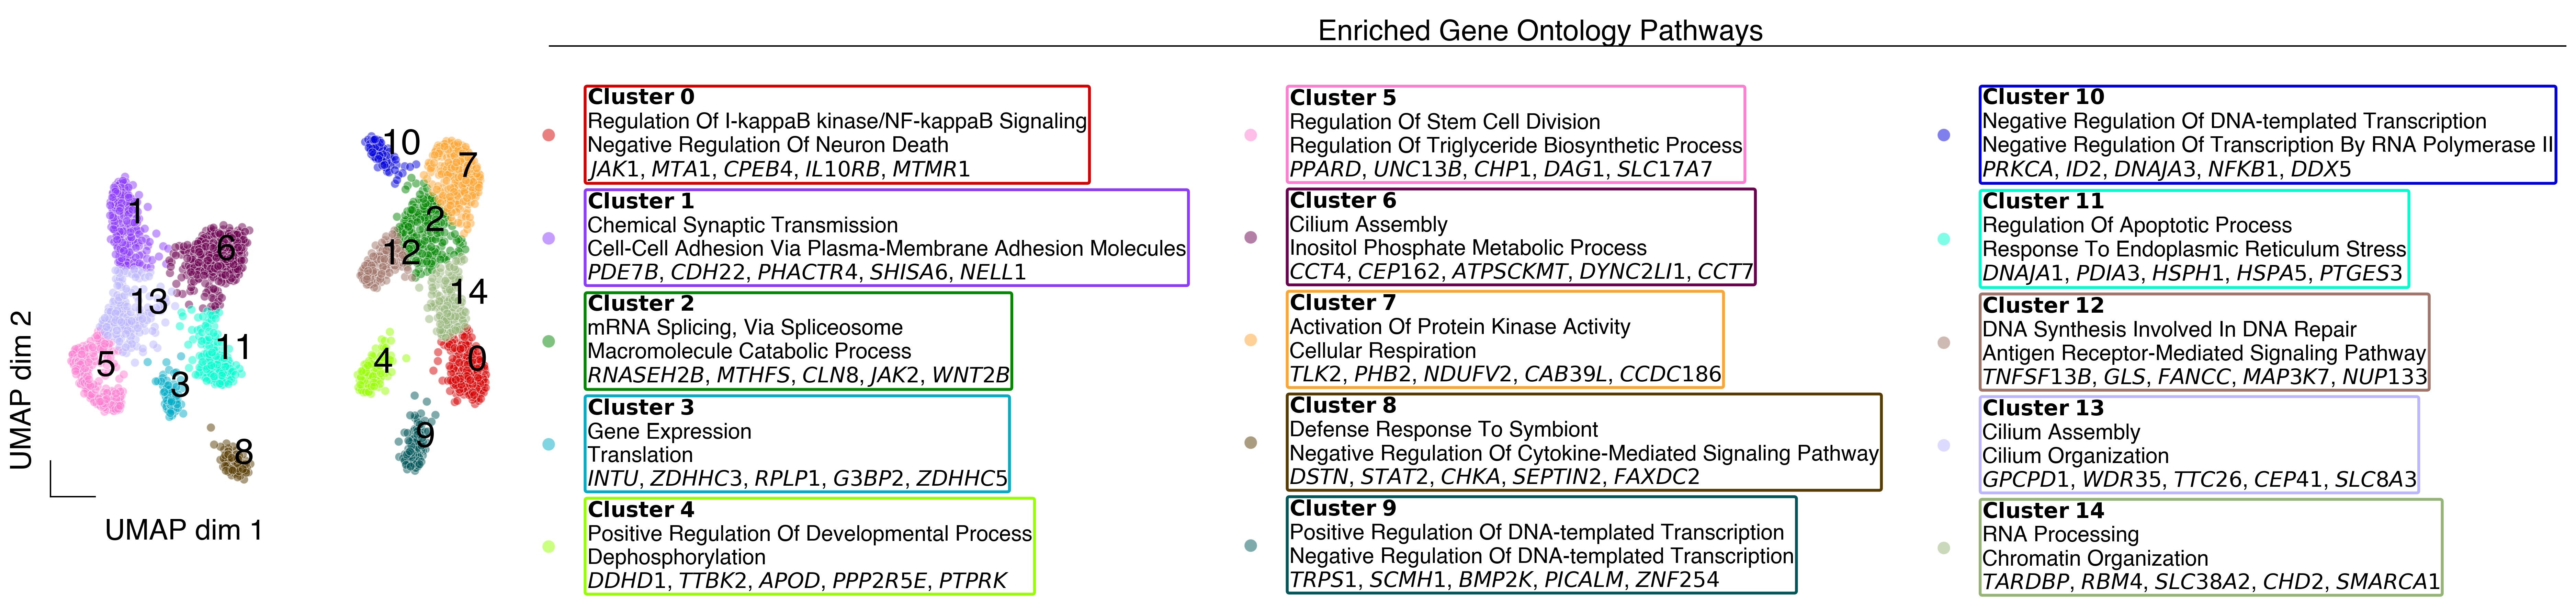
\includegraphics[width=\textwidth]{./main_plots/clusters_umap.png}        
    \end{subfigure}
    \\[-2ex] 
    \begin{subfigure}[t]{\textwidth}
        \caption{}
        
\includegraphics[width=\textwidth]{./main_plots/clusters_bars.png}        
    \end{subfigure}
    \caption{
        \textbf{Single-nuclear RNA-sequencing Atlas of Human Post-mortem Prefrontal Cortex Reveals Cell Type-specific Gene Changes in ABCA7 LoF.}\\[1ex]
        (A) Overview of ABCA7 gene structure with the location of variants represented in this study (average minor allele frequency for depicted variants is < 1\%). Exons are depicted as black rectangles, and introns as black lines. The pie chart indicates the frequency of ABCA7 PTC-variant-carriers within the ROSMAP cohort. 
        (B) ABCA7 protein levels (log2(abundance)) from post-mortem human prefrontal cortex in all available controls ($N=180$) vs. ABCA7 LoF carriers ($N=5$). P-value computed by Wilcoxon rank sum test. Boxes indicate per-condition dataset quartiles, and whiskers extend to the most extreme data points not considered outliers (i.e., within 1.5 times the interquartile range from the first or third quartile). 
        (C) Overview of human cohort for snRNA-seq (Created with BioRender.com). 
        (D) Overview of snRNA-seq cohort metadata for 32 individuals. 
        (E) 2D UMAP projection of per-cell gene expression values and their transcriptionally defined cell type. 
        (F) 2D UMAP projection of ABCA7 LoF gene perturbation scores ($S = -\log_{10}(\text{p-value}) \times \text{sign}(\log_2(\text{fold change}))$); Red = $S>1.3$, Blue = $S<-1.3$; Point size indicates $|S|$). Up to top 20 genes by $|S|$ are labeled. 
        (G) Genes in 2D UMAP space colored by cluster assignment (Gaussian mixture model; see Methods) with per-cluster pathway enrichments shown (GO BP, hypergeometric enrichment, $p<0.01$). 
        (H) Cell type-specific gene cluster scores ($SC = \text{mean}(S_i)$, for genes $i$ in cluster $c$). * indicates permutation FDR-adjusted p-value $< 0.01$ and $|SC| > 0.25$.
    }
    \label{fig:main_atlas}
\end{figure}